% StrainWTDataSet_RightWing.tex

\tikzstyle{RectObject}=[rectangle,draw=blue,rounded corners,line width=0.5mm,
  minimum width=6em,minimum height=10em]
\tikzstyle{LinStrainObject}=[draw=blue,rounded corners,line width=0.5mm]
\tikzstyle{LabelObject}=[fill=white,rectangle,rounded corners,line width=0.5mm,%
	align=center]
\tikzstyle{ArrowObject}=[red,line width=1.0mm, -latex]

\resizebox{!}{0.45\textwidth}{
	\begin{tikzpicture}
		\node[anchor=south west,inner sep=0] (image) at (0,0)%
			{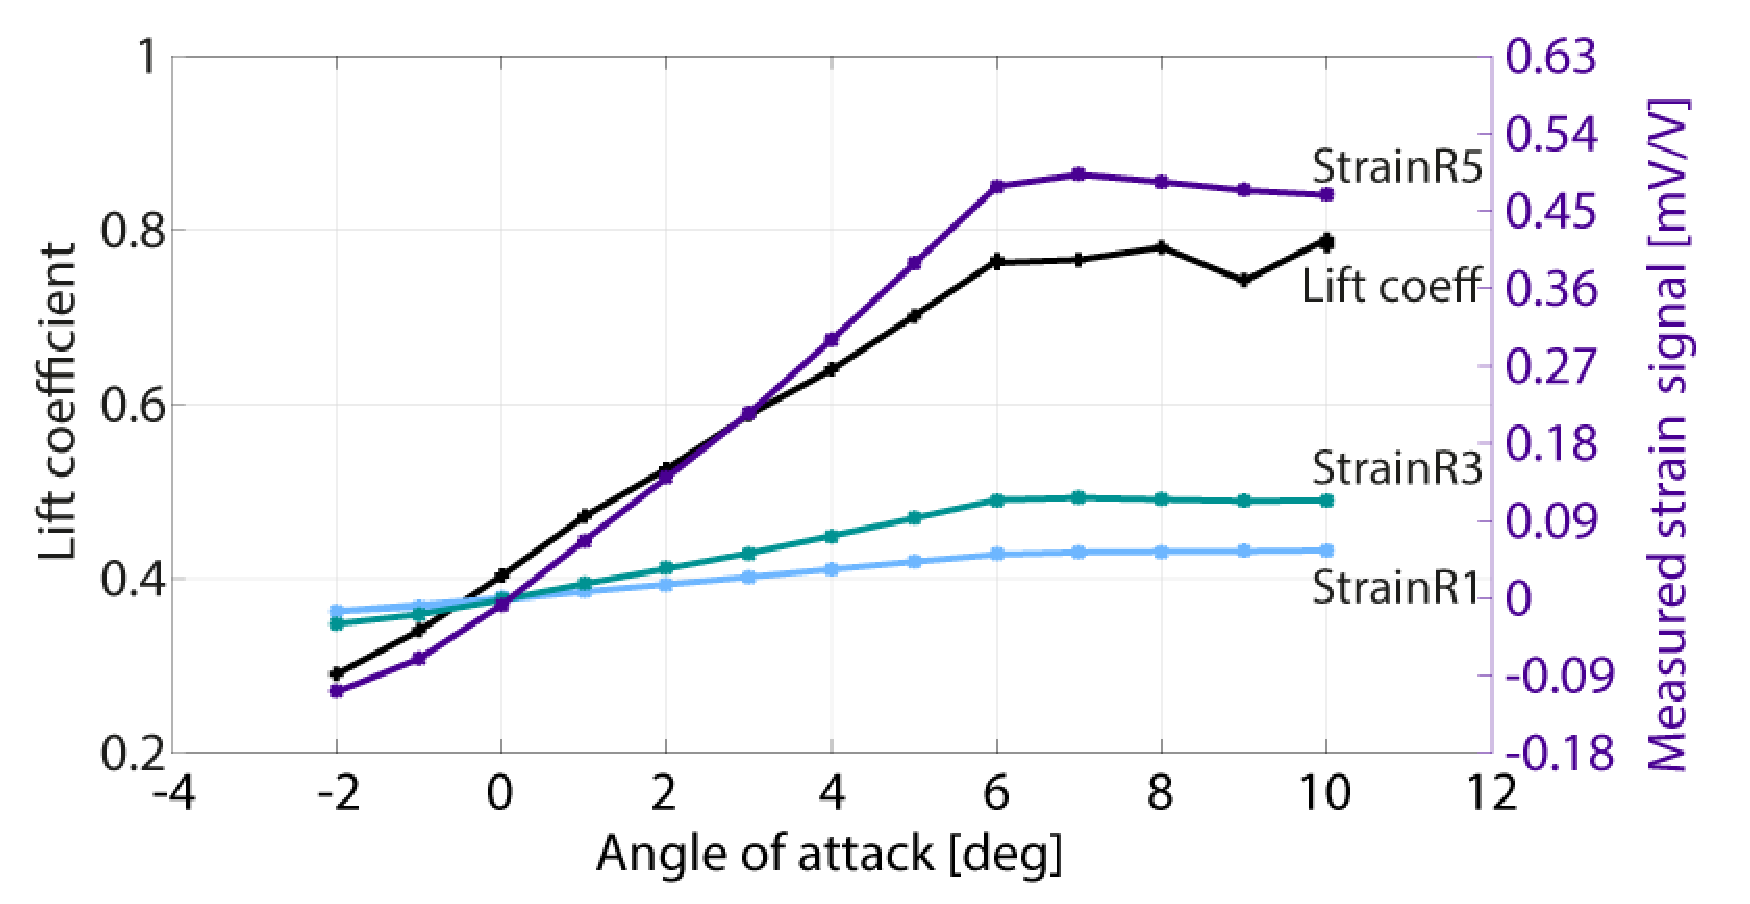
\includegraphics[width=\textwidth]{StrainWTDataSet_RightWing.eps}};
		% Define scope with 'image' dimensions as reference
		\begin{scope}[x={(image.south east)},y={(image.north west)}]
			%\draw[help lines,xstep=.05,ystep=.05] (0,0) grid (1,1);
			%\foreach \x in {0,1,...,9} { \node [anchor=north] at (\x/10,0) {0.\x}; }
			%\foreach \y in {0,1,...,9} { \node [anchor=east] at (0,\y/10) {0.\y}; }
			
			% Aircraft diagram
			\node[anchor=south west,inner sep=0] (AircraftDiagram) at (0.1,0.6)%
			  {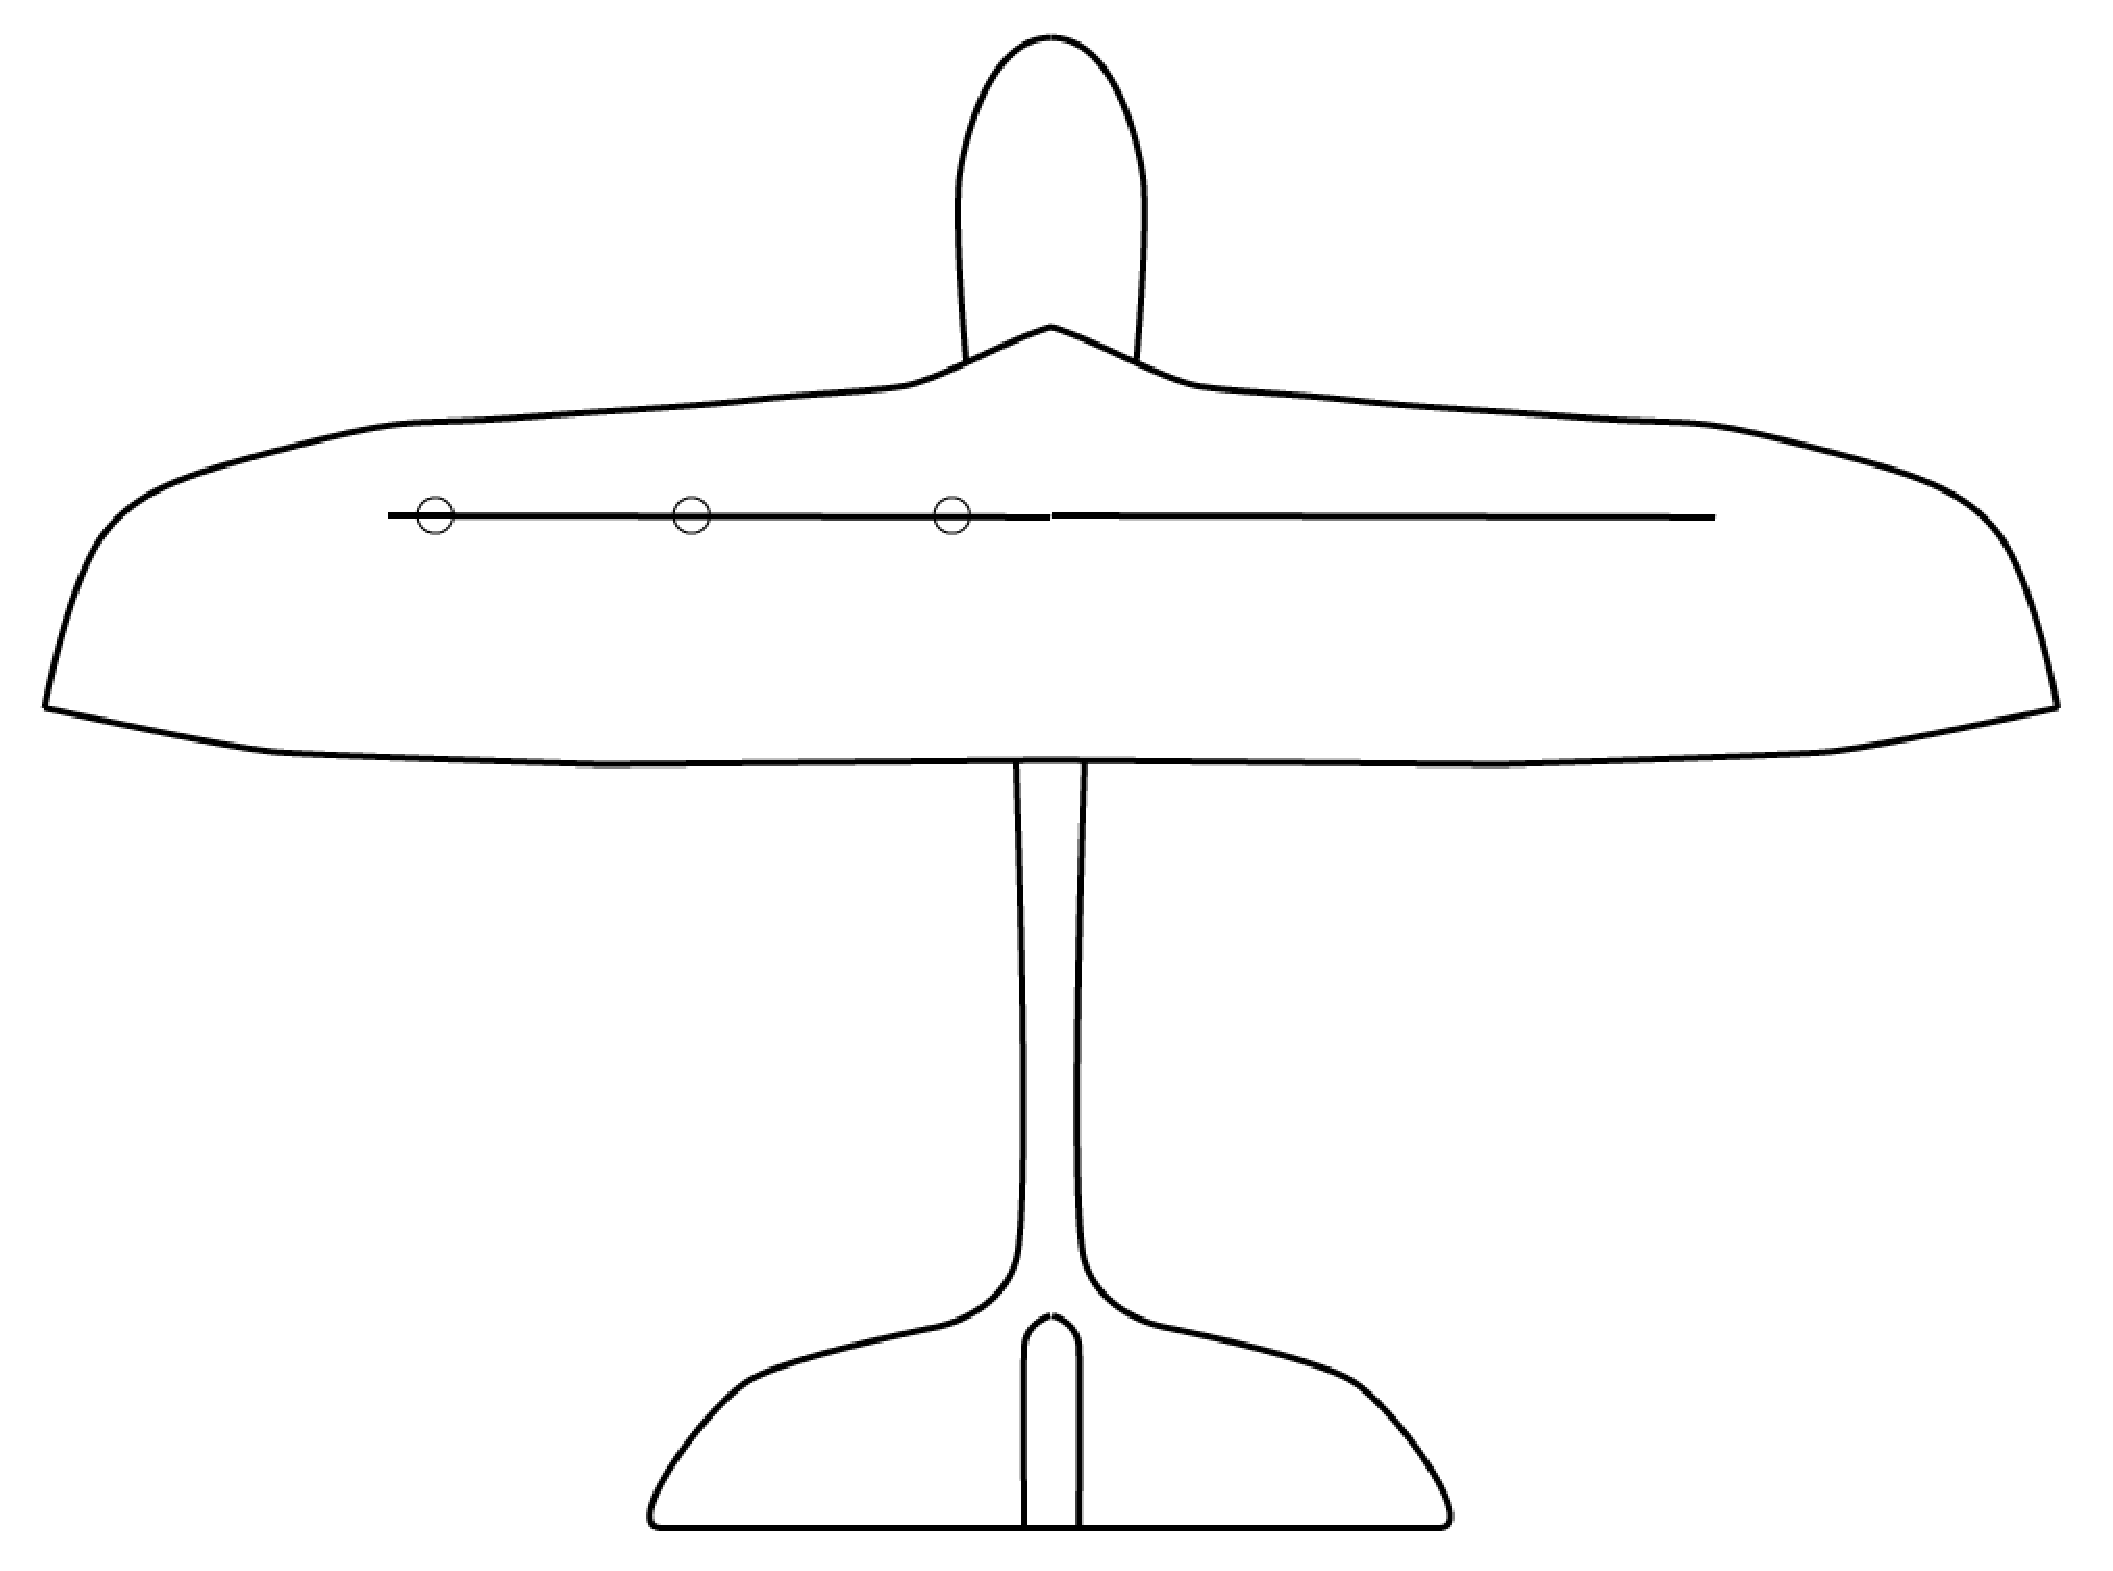
\includegraphics[width=0.25\textwidth]{EasySkyOutline.eps}};
			% Strain sensors on aircraft
			\draw(AircraftDiagram) ++(-0.011, 0.0625) node[mark size=1pt,color=violet] (SR1) {\pgfuseplotmark{*}};
			\draw(AircraftDiagram) ++(-0.045, 0.0625) node[mark size=1pt,color=black!50!green]  (SR2) {\pgfuseplotmark{*}};
			\draw(AircraftDiagram) ++(-0.075, 0.0625) node[mark size=1pt,color=cyan]   (SR3) {\pgfuseplotmark{*}};
			
			\only<4>{
			  % Linear Strain with AoA
			  \draw[LinStrainObject] (0.55,0.20) -- (0.55,0.50) node[anchor=east] (ForArrow) {}
			    -- (0.55,0.80) -- (0.10,0.20) -- cycle;
			  % Linear Strain with AoA label
			  \draw(0.7,0.2) node[LabelObject] (LinStrain_Label) {Linear Strain\\With AoA};
			  % Linear Strain with AoA arrow
			  \draw[ArrowObject] (LinStrain_Label.north) -- (ForArrow.east);
			}
			\only<5>{
			  % Strain Stall Markers
			  \draw(0.66,0.55) node[RectObject] (StrainStall) {};
			  % Strain Stall Markers label
			  \draw(0.30,0.30) node[LabelObject] (StrainStall_Label)
				  {Large increase\\in variance\\ during stall};
			  % Strain Stall Markers arrow
			  \draw[ArrowObject] (StrainStall_Label.north east) -- (StrainStall.west);
			}
			
		\end{scope}
  \end{tikzpicture}
}